\documentclass{article}

\usepackage{tikz}
\usetikzlibrary{matrix,chains,positioning,decorations.pathreplacing,arrows}
\usepackage{minted}

\addtolength{\oddsidemargin}{-.875in}
\addtolength{\evensidemargin}{-.875in}
\addtolength{\textwidth}{1.75in}

\addtolength{\topmargin}{-.875in}
\addtolength{\textheight}{1.75in}

\bibliographystyle{plain}

\begin{document}

\title{An Exploration of Neural Networks as Applied to Written Language Classification}
\author{Erik Boesen, Candidate [Number]}

\maketitle

\begin{abstract}
We assess the extent to which artificial neural networks can be used to perform recognition of written languages (conveyed through standard Unicode text rather than as graphically recognized handwriting). We use an artificial deep neural network to achieve a success rate of [Insert] at distinguishing between 8 different languages following supervised training.
\end{abstract}

\section{Introduction}
In this research we seek to develop and implement (using C++) a neural network which differentiates between the world's 8 most common first languages according to \cite{ethnologue}, namely: Chinese, Spanish, English, Arabic, Hindi, Bengali, Portuguese, and Russian (ISO 639-2 bibliographic alpha-3 codes chi, spa, eng, hin, ben, por, rus) \cite{iso639}.

\subsection{Training Data}
To train our network, we use dumps of article contents in the selected languages from the Wikimedia Foundation, obtained from \cite{wikidumps} as recommended in \cite{langsamp}. % Remove second citation?

\section{A general overview of neural networks}
\subsection{Why use Neural Networks?}
Neural Networks (NNs) are a common technique used in Machine Learning (ML). ML techniques are useful when a large and diverse set of data must be processed (often entailing categorization), but when writing explicit code to make distinctions between data points would be impractical. For example, when identifying objects in an image, as in \cite{hinton12}, it would be nearly impossible to write a procedure to directly read image data and distinguish between many images. Though there exist simpler ML techniques, such as the K Nearest Neighbors algorithm, these strategies have trouble making decisions in so many dimensions with such a complex output vector as demonstrated in \cite{knnic}.

\subsection{Structure}
% TODO: This explanation is insufficient.
Neural Networks make tasks like the aforementioned easier by taking cues from neurobiology and simulating how a real brain makes decisions. Virtual neurons are chained together in layers.

The process performed by each neuron during training is relatively simple. First, the neuron sums the output values of all previous neurons, including the bias neuron, multiplied by their weights. It then passes the result through an activation function, such as the sigmoid function, to bring the output into the range $(0, 1)$ (or, for activation functions like $tanh(x)$, $(-1, 1)$).

\begin{figure}
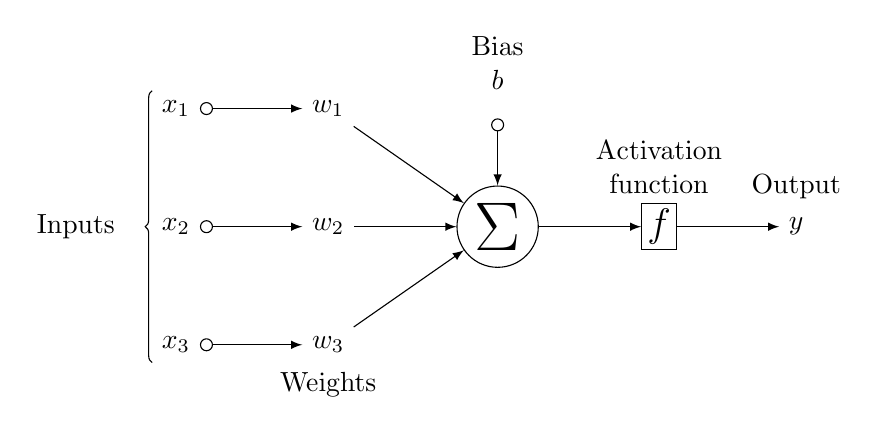
\begin{tikzpicture}[
init/.style={
  draw,
  circle,
  inner sep=2pt,
  font=\Huge,
  join = by -latex
},
squa/.style={
  draw,
  inner sep=2pt,
  font=\Large,
  join = by -latex
},
start chain=2,node distance=13mm
]
\node[on chain=2]
  (x2) {$x_2$};
\node[on chain=2,join=by o-latex]
  {$w_2$};
\node[on chain=2,init] (sigma)
  {$\displaystyle\Sigma$};
\node[on chain=2,squa,label=above:{\parbox{2cm}{\centering Activation \\ function}}]
  {$f$};
\node[on chain=2,label=above:Output,join=by -latex]
  {$y$};
\begin{scope}[start chain=1]
\node[on chain=1] at (0,1.5cm)
  (x1) {$x_1$};
\node[on chain=1,join=by o-latex]
  (w1) {$w_1$};
\end{scope}
\begin{scope}[start chain=3]
\node[on chain=3] at (0,-1.5cm)
  (x3) {$x_3$};
\node[on chain=3,label=below:Weights,join=by o-latex]
  (w3) {$w_3$};
\end{scope}
\node[label=above:\parbox{2cm}{\centering Bias \\ $b$}] at (sigma|-w1) (b) {};

\draw[-latex] (w1) -- (sigma);
\draw[-latex] (w3) -- (sigma);
\draw[o-latex] (b) -- (sigma);

\draw[decorate,decoration={brace,mirror}] (x1.north west) -- node[left=10pt] {Inputs} (x3.south west);
\end{tikzpicture}
\caption{A diagram of a single neuron.} \label{fig:M1}
\end{figure}

Each neural network contains three types of layers, or vectors of neurons:
\begin{itemize}
\item{Input Layer - Neurons which directly recieve input values.}
\item{Hidden Layers - Input data is fed through one or more of these, which multiply values by various weights (notated $\omega_n$) in order to arrive at a final "output layer," which contains the data desired by a user.}
\item{Output Layer - A vector of output values.}
\end{itemize}

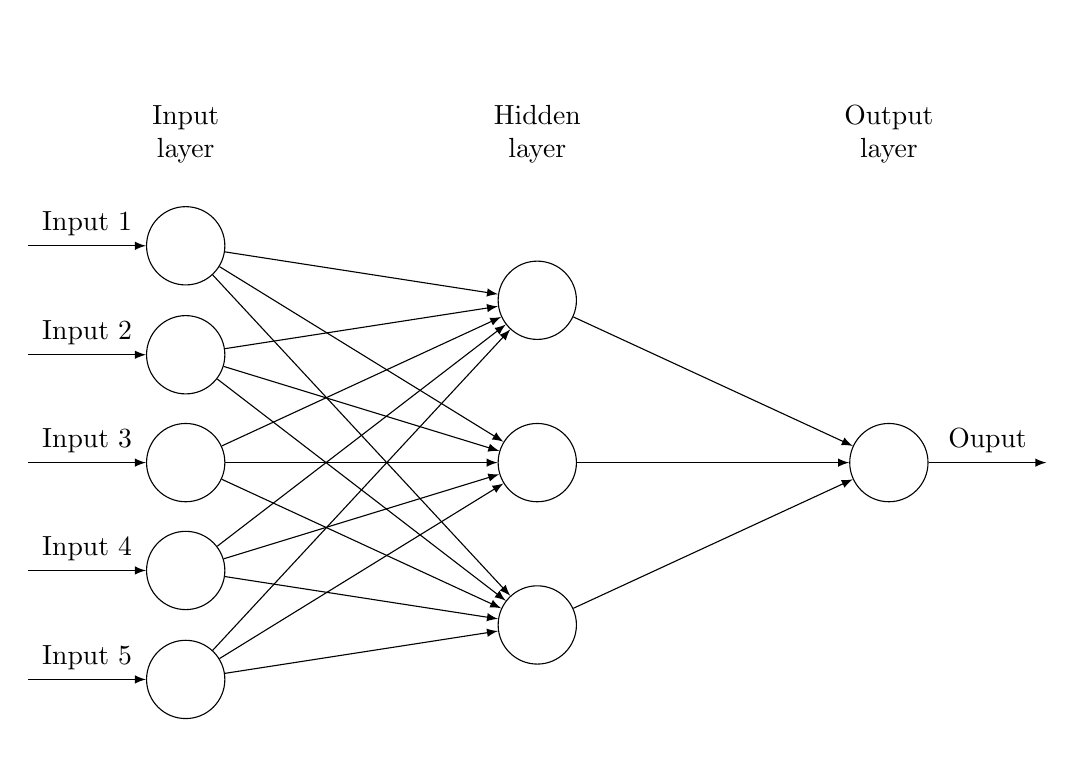
\begin{tikzpicture}[
plain/.style={
  draw=none,
  fill=none,
  },
net/.style={
  matrix of nodes,
  nodes={
    draw,
    circle,
    inner sep=10pt
    },
  nodes in empty cells,
  column sep=2cm,
  row sep=-9pt
  },
>=latex
]
\matrix[net] (mat)
{
|[plain]| \parbox{1.3cm}{\centering Input\\layer} & |[plain]| \parbox{1.3cm}{\centering Hidden\\layer} & |[plain]| \parbox{1.3cm}{\centering Output\\layer} \\
& |[plain]| \\
|[plain]| & \\
& |[plain]| \\
  |[plain]| & |[plain]| \\
& & \\
  |[plain]| & |[plain]| \\
& |[plain]| \\
  |[plain]| & \\
& |[plain]| \\    };
\foreach \ai [count=\mi ]in {2,4,...,10}
  \draw[<-] (mat-\ai-1) -- node[above] {Input \mi} +(-2cm,0);
\foreach \ai in {2,4,...,10}
{\foreach \aii in {3,6,9}
  \draw[->] (mat-\ai-1) -- (mat-\aii-2);
}
\foreach \ai in {3,6,9}
  \draw[->] (mat-\ai-2) -- (mat-6-3);
\draw[->] (mat-6-3) -- node[above] {Ouput} +(2cm,0);
\end{tikzpicture}

\subsection{Backpropogation}
A central component of neural network training is the backpropogation algorithm. In this

\section{Technical stack}
For implementing our network we use C++. However, given that the general logic of the network could be implemented in practically any language, we use the most simplistic implementation possible; avoiding excessive use of C++-specific idioms. Any opaque logic is explained. Syntax highlighting is provided as well for ease of use:
\begin{minted}{cpp}
#include <iostream>

using namespace std;
int main(int argc, char *argv[]) {
    cout << "Hello world!" << endl;
}
\end{minted}

\bibliography{research}

\end{document}
